%%%  _____               _
%%% |_   _|__  ___  _ __(_) __ _
%%%   | |/ _ \/ _ \| '__| |/ _` |
%%%   | |  __/ (_) | |  | | (_| |
%%%   |_|\___|\___/|_|  |_|\__,_|
%%%
%%% TCC de Bianca Miyabe Santos Freitas
%%% Licenciatura em Física - UFSCar, Sorocaba
%%%

\chapter{Fundamentação Teórica}

Conforme descrito no Capítulo de Introdução, para o estudo da Computação Quântica e da Informação Quântica são necessários alguns recursos provenientes da MQ, bem como a construção de análogos quânticos para o processamento dessa informação. As seções a seguir apresentarão a fundamentação teórica e os recursos matemáticos necessários para o desenvolvimento da simulação proposta na Metodologia.

\section{Conceitos básicos de Álgebra Linear}\label{sec:algelin}
A Álgebra Linear é o estudo dos vetores que descrevem um espaço e consequentemente das operações nesses espaços vetoriais. Para o desenvolvimento desse trabalho, serão necessários reconhecer as notações descritas na Tabela~\ref{tab:notação}.

\begin{table}[ht!]
  \centering
  \caption{Notações utilizadas nas operações de MQ e sua respectiva descrição. O estilo das notações é conhecido como Notação de Dirac para Álgebra Linear.}\label{tab:notação}
  \begin{tabular}{cl}
    \toprule
    {\textbf{Notação}}                 & {\textbf{Descrição}}                                                 \\
    \midrule
    $\ket{\psi}$                       & Vetor conhecido como \textit{ket}                                    \\
    $\bra{\psi}$                       & Vetor dual de um \textit{ket} conhecido como \textit{bra}            \\
    $\braket{\psi\vert\varphi}$        & Produto interno entre os vetores $\ket{\psi}$ e $\ket{\varphi}$      \\
    $\ket{\psi} \otimes \ket{\varphi}$ & Produto tensorial entre os vetores $\ket{\psi}$ e $\ket{\varphi}$    \\
    $\ket{\psi}\ket{\varphi}$          & Abreviação do produto tensorial entre $\ket{\psi}$ e $\ket{\varphi}$ \\
    $A^*$                              & Conjugado complexo da matriz \(A\)                                   \\
    \bottomrule
  \end{tabular}
  \fonte{Adaptada de \textcite{chuang}.}
\end{table}

A descrição da MQ é feita tomando como base um espaço vetorial chamado \textit{Espaço de Hilbert} $\mathcal{H}$, sendo este um espaço complexo, vetorial e linear. Um \textit{ket} é um vetor arbitrário de $\mathcal{H}$, com representação descrita por:
\begin{equation}\label{eq:ketpsi}
  \ket{\psi} = [\psi_1,...,\psi_n]^T \in \mathcal{H}.
\end{equation}

Todo \textit{ket} possui um vetor dual, ou conjugado complexo que também pertence à $\mathcal{H}$, chamado de \textit{bra}, de modo que:
\begin{equation}\label{eq:brapsi}
  \bra{\psi} = [\psi_1^*,...,\psi_n^*] \in \mathcal{H}.
\end{equation}

O produto tensorial entre dois \textit{kets} \(\ket{\psi}\) de dimensão \(m\) e \(\ket{\varphi}\) de dimensão \(n\) é definido por:

\begin{equation}\label{eq:tensorket}
  \begin{split}
    \ket{\psi} \otimes \ket{\varphi} &= \ket{\psi}\ket{\varphi} =\ket{\psi \varphi} = \\
    &=\scalebox{0.9}{\(\begin{pmatrix}\psi_1 \varphi_1 & \psi_1 \varphi_2 & \cdots & \psi_1 \varphi_n & \psi_2 \varphi_1 & \psi_2 \varphi_2 & \cdots & \psi_2 \varphi_n & \cdots & \psi_m \varphi_2 & \psi_m \varphi_2 & \cdots & \psi_m \varphi_n\end{pmatrix}^{T}\)}.
  \end{split}
\end{equation}
Podemos também realizar o produto tensorial de duas matrizes \(A\in\mathbb{C}^{m{\times}n}\) e \(B\in\mathbb{C}^{p{\times}q}\), de modo que:
\begin{equation}\label{eq:tensormatrix}
  A \otimes B = \begin{pmatrix}
                  A_{11} B  & A_{12} B  & \cdots & A_{1 n} B \\
                  A_{21} B  & A_{22} B  & \cdots & A_{2 n} B \\
                  \vdots    & \vdots    & \ddots & \vdots    \\
                  A_{m 1} B & A_{m 2} B & \cdots & A_{m n} B
                \end{pmatrix}_{m p \times n q}.
              \end{equation}

O conjugado complexo de uma matriz é definido como a matriz transposta dos seus elementos conjugados, de modo que:
\begin{equation}\label{eq:conjugadomatrix}
  A^{\!*} = \begin{pmatrix}
                a & b \\
                c & d
          \end{pmatrix}^{\!\!\!*} =
          \begin{pmatrix}
            a^{*} & c^{*} \\
            b^{*} & d^{*}
          \end{pmatrix}.
      \end{equation}

Os recursos apresentados acima, serão utilizados ao longo do trabalho e principalmente na descrição da Seção~\ref{sec:Mecanicaquantica}.


\section{Mecânica Quântica}\label{sec:Mecanicaquantica}

A teoria da Física intitulada Mecânica Quântica (MQ), surgiu no século XX após uma série de experimentos constatarem que as leis físicas conhecidas até então, não se aplicavam em sistemas da ordem de 1 \AA, ou seja, $10^{-10}m$. Com o avanço dos estudos e experimentos na MQ, foi possível tornar 'visível' uma série de comportamentos da Natureza que antes eram observados apenas em escala macroscópica. Esse aumento na capacidade da descrição da Natureza só foi possível devido a uma série de ferramentas matemáticas e axiomas que constituem a teoria da MQ \cite{jorcuvich}. 

A compreensão dessa teoria física, não foi aceita pela comunidade científica assim que foi sugerida, por volta de 1925, com os trabalhos de vários cientistas, como Max Planck, Albert Einstein, Niels Bohr, Werner Heisenberg, Erwin Schrödinger, entre outros\footnote{Um descrição detalhada dos experimentos e evoluções conceituais que culminaram na estrutura da MQ que conhecemos na atualidade pode ser encontrada no artigo de \textcite{chibeni}.}, principalmente pelo fato de que, naquela época, os recursos tecnológicos para o desenvolvimento de experimentos que confirmassem a teoria proposta era ainda escassa.\cite{chibeni}. 

Até mesmo Albert Einstein duvidava de alguns aspectos da teoria, como exemplo, conforme veremos nos próximos capítulos, o fenômeno de Emaranhamento Quântico causava em Einstein certa estranheza, em suas próprias palavras "Uma ação fantasmagórica à distância", era a melhor descrição para o fenômeno. O fato da MQ não ser observada diretamente ainda causa estranheza, porém, isso não a torna menos correta que qualquer outra teoria, pelo contrário, atualmente a MQ é considerada uma das teorias mais completas utilizadas para a descrição da Natureza \cite{chuang}. Nas próximas seções, alguns conceitos da MQ serão apresentados para a compreensão do desenvolvimento do trabalho, baseando-se principalmente nas ideias apresentadas por \textcite{chuang,jorcuvich,CompInfoQuantica,grif}.


\subsection{Postulados da MQ}\label{sec:postulados}

Os postulados descritos abaixo norteiam a construção das próximas seções. Cada um deles descreve uma característica fundamental da MQ, que posteriormente será utilizada na construção do trabalho.

\begin{post}{Espaço de estados}{p1}
Considerando todo e qualquer sistema físico que esteja isolado, os estados do sistema estão associados à um espaço de Hilbert $\mathcal{H}$ e podem ser descritos por um vetor de estado unitário $\ket{\psi} \in \mathcal{H}$.
\end{post}

\begin{post}{Evolução}{p2}
Ainda considerando um sistema físico isolado, sua evolução, ou seja, sua mudança é descrita por uma transformação unitária, ou seja, para que um sistema mude do estado $\ket{\psi}$ para $\ket{\psi'}$, é necessário que atue sobre ele um operador unitário (que pode ser representado por uma matriz) \textit{U}, de modo que $\ket{\psi'}=\textit{U}\ket{\psi}$. Uma consequência é que a aplicação de um operador unitário, mantém a norma unitária do estado como definido pelo Postulado 1. Outra consequência é que todo operador unitário é inversível, o que implica que as operações quânticas são reversíveis.
\end{post}

\begin{post}{Medição}{p3}
Quando um sistema quântico é medido, o resultado da medição é um dos possíveis valores permitidos pelo sistema e a probabilidade de obter cada valor depende do estado do sistema antes da medição. Em outras palavras, quando um sistema quântico é medido, ele colapsa em um dos estados possíveis fazendo com que a medição altere o estado do sistema. 
\end{post}

\begin{post}{Composição dos estados}{p4}
Um espaço de estado de um sistema quântico composto é descrito pelo produto tensorial dos dos espaços de estado que o compõem. Por exemplo, seja o estado quântico $\ket{\Psi}$ composto pelos espaços de estado $\ket{\psi_1}, \ket{\psi_2} e \ket{\psi_3}$, podemos descrevê-lo como 
\begin{equation}
\ket{\Psi}=\ket{\psi_1} \otimes \ket{\psi_2} \otimes \ket{\psi_3} = \ket{\psi_1}\ket{\psi_2}\ket{\psi_3}
\end{equation}
\end{post}

\subsection{Superposição de Estados}\label{sec:superposição}

A superposição de estados quânticos é uma característica fundamental da MQ que descreve o comportamento de sistemas quânticos em termos de estados que são combinados linearmente. Em outras palavras, quando um sistema quântico está em um estado de superposição, ele está simultaneamente em vários estados possíveis, cada um com uma probabilidade associada.

Essa característica é fundamental para a existência dos qubits conforme veremos na seção~\ref{sec:qubits}. Quando um sistema quântico é medido, ele colapsa em um estado único e observável, conforme explicitado no Postulado~\ref{post:p3}. Isso é conhecido como o colapso da função de onda e a probabilidade de medir cada estado possível é determinada pelas amplitudes de probabilidade associadas aos estados na superposição.

A superposição de estados quânticos é uma das características mais estranhas e fascinantes da MQ e permite o acontecimento de fenômenos como como o emaranhamento quântico e o teletransporte quântico.


\subsection{Emaranhamento Quântico}\label{sec:emaranhamento}

O Emaranhamento quântico é uma propriedade da MQ que descreve a correlação entre dois ou mais sistemas quânticos, de tal forma que o estado quântico de um  não pode ser descrito independentemente do estado dos outros sistemas emaranhados.

O emaranhamento quântico tem implicações importantes, como por exemplo, no caso da comunicação quântica que utiliza o emaranhamento quântico para transmitir informações de forma segura, pois qualquer tentativa de interceptar a comunicação alteraria o estado emaranhado e seria detectável.

O emaranhamento quântico também é importante na computação quântica, onde os qubits emaranhados podem ser usados para executar operações de forma mais rápida e eficiente do que seria possível com qubits individuais. Além disso, o emaranhamento quântico tem aplicações em áreas como a criptografia quântica, a simulação quântica e a teletransporte quântico.

Para compreender melhor esse fenômeno, podemos pensar na situação onde temos um sistema de dois qubits $\ket{\psi}=\alpha\ket{0}+\beta\ket{1}$ e $\ket{\varphi}=\mu\ket{0}+\eta\ket{1}$. Se em nosso sistema, os dois qubits são independentes, significa que possuirão probabilidades associadas aos estados $\ket{0}$ e $\ket{1}$ distintas, ou seja, $\alpha \neq \beta \neq \mu \neq \eta$. Considerado agora que os qubits $\ket{\psi}$ e $\ket{\varphi}$ estejam emaranhados, os estados não poderão ser mais considerados de forma independente e portanto, as probabilidades são descritas associadas aos estados possívei. Teremos portanto, os estados emaranhados $\ket{00}, \ket{01}, \ket{10} e \ket{11}$ cujas probabilidades dependerão de ambos os qubits. Alterando os estados de um qubit, consequentemente o outro será alterado, fazendo com que passemos a pensar numa distribuição de probabilidade entre os estados. Um processo simplificado da utilização do emaranhamento em computação quântica pode ser encontrado em \ref{list:emaranhamento}.

\textbf{Etapas do Emaranhamento Quântico de Qubits}

\begin{itemize}\label{list:emaranhamento}
\item 1. Preparação:  O primeiro passo é preparar os qubits individuais. Isso pode ser feito carregando os qubits em computadores quânticos ou usando dispositivos quânticos especializados, como lasers.

\item 2. Entrelaçamento: Em seguida, os qubits são entrelaçados, o que significa que eles são interconectados de modo que as informações entre eles sejam compartilhadas. Isso pode ser feito usando técnicas como a interferência quântica.

\item 3. Operações: Uma vez que os qubits estão entrelaçados, as operações quânticas podem ser realizadas neles. As operações podem incluir a realização de computações quânticas complexas, o armazenamento de informações quânticas ou o envio de informações entre qubits.

\item 4. Saída: Por fim, os qubits podem ser desentrelaçados para obter a saída desejada. A saída pode incluir informações codificadas nos qubits, como um resultado de uma computação quântica.
\end{itemize}

\subsection{Teorema da Não-Clonagem}\label{sec:naoclonagem}

O teorema da não-clonagem de qubits é um resultado fundamental na teoria da informação quântica que afirma que é impossível fazer uma cópia exata do estado quântico de um qubit arbitrário. Em outras palavras, não é possível criar uma máquina de clonagem quântica que produza uma cópia idêntica de um qubit desconhecido, diferente da informação clássica que pode ser facilmente reproduzida, basta recordar que um livro pode ser impresso com a tiragem de exemplares desejada.

Esse resultado tem implicações importantes para a criptografia quântica e a segurança da comunicação quântica, pois impede a interceptação e a cópia dos estados quânticos usados para transmitir informações. O teorema da não clonagem foi provado por Wooters e Zurek em 1982, e é um dos resultados fundamentais da teoria da informação quântica \cite{clone}.

Uma das implicações interessantes do teorema da não-clonagem é que a medição de um qubit não é apenas uma operação de leitura, mas também uma operação de destruição do estado quântico. Em outras palavras, ao medir um qubit, o estado quântico original é destruído e uma das possíveis informações clássicas é obtida. 

Podemos formalizar o teorema da seguinte forma:

\begin{theo}{Não-Clonagem}{clone}
Seja $\mathcal{H}$ um espaço de Hilbert, não existe transformação que torne possível a seguinte expressão:
\begin{equation}
U:\mathcal{H} \otimes \mathcal{H} \rightarrow \mathcal{H} \otimes \mathcal{H}
\end{equation}
\end{theo}

\subsection{Paradoxo EPR}\label{sec:epr}

O Paradoxo EPR é um famoso argumento em favor da incompletude da MQ, proposto por Albert Einstein, Boris Podolsky e Nathan Rosen em 1935. O paradoxo começa com a observação de que a MQ prevê que duas partículas emaranhadas podem estar em um estado quântico compartilhado, mesmo que estejam distantes uma da outra.

De acordo com a MQ, se duas partículas são emaranhadas, a medição do estado quântico de uma partícula instantaneamente afetará o estado quântico da outra partícula, independentemente da distância entre elas. Isso significa que as partículas emaranhadas parecem estar em comunicação instantânea, o que violaria a teoria da relatividade especial de Einstein, que proíbe a comunicação mais rápida do que a velocidade da luz.

Einstein, Podolsky e Rosen propuseram um experimento mental para demonstrar essa aparente contradição. No experimento, duas partículas emaranhadas são criadas e separadas a uma grande distância uma da outra. Em seguida, uma propriedade quântica específica de uma das partículas é medida, o que instantaneamente afeta a propriedade quântica da outra partícula, mesmo que esteja a uma grande distância. Isso parece violar a teoria da relatividade especial de Einstein, que proíbe a comunicação mais rápida do que a velocidade da luz.

A resolução do paradoxo EPR veio da própria teoria da MQ e sua interpretação correta. A MQ não viola a relatividade especial de Einstein, pois as partículas emaranhadas não estão realmente em comunicação instantânea, em vez disso, o estado quântico das partículas emaranhadas é uma superposição de estados possíveis e a medição do estado de uma das partículas colapsa a função de onda do sistema emaranhado como um todo, fazendo com que o estado da outra partícula pareça estar sendo afetado instantaneamente. A explicação correta é que a medição da primeira partícula, que afeta instantaneamente a segunda partícula, não é uma ação física, mas sim uma consequência da natureza probabilística da MQ.


\subsection{Teletransporte Quântico}\label{sec:teletransporteteoria}

O Teletransporte Quântico consiste em uma série de operações realizadas por intermédio de um circuito de natureza quântica que pretende enviar uma mensagem de um ponto \(A\) até um ponto \(B\). Ele consiste em uma série de operações que possibilitam descrever no ponto \(B\) um estado existente no ponto \(A\). A princípio, devido ao Teorema da Não-Clonagem (~\ref{sec:naoclonagem}), seria impossível ``clonar'' um estado quântico, ou seja, teletransportar a informação de modo semelhante ao que ocorre com um canal clássico. Porém, segundo \textcite{bennet}, é possível contornar o problema utilizando um canal de informação clássico, semelhante ao apresentado por Shannon na TMC, porém utilizando como emissor-receptor um par de partículas emaranhadas quanticamente.

Na literatura encontram-se as mais diversas explicações sobre como funciona o teletransporte quântico \cites{bennet}{experimentalqt}{zeilinger}{brassard1996teleportation}{materialdidaticomecquantica} e na maioria dos casos, os leitores são introduzidos a dois personagens: Alice e Bob.

Na história, os cientistas Alice e Bob estão localizados em dois laboratórios distintos, cada um deles possui uma partícula, ${A}$ e ${B}$ e estas estão emaranhadas, produzindo um estado quântico emaranhado denominado de $\ket{\psi_{AB}}$. Alice precisa enviar uma mensagem urgente para Bob utilizando um outro estado, ${C}$. Portanto, no início do processo de teletransporte, Alice possui dois estados, o que ela deseja enviar e o que está emaranhado com o Bob.

Alice realiza então uma série de operações entre suas partículas e para continuar o processo de teletransporte, faz uma medição, colapsando-as e envia, via um canal clássico, a informação dos estados colapsados para Bob. Este por sua vez, por saber qual era o estado inicial de ${A}$ devido ao emaranhamento, consegue reconstruir a mensagem presente originalmente em ${C}$ enviado por Alice. Portanto, a mensagem é reconstruída e não clonada, não violando o princípio da não-clonagem. A não-clonagem fica explicitada no momento em que a medida é realizada em ${A}$ e ${C}$, colapsando-os, de modo que existe apenas uma cópia do estado de ${C}$ dado por $\ket{\psi_{C}}$.


\section{Computação Quântica}\label{sec:compquant}
As definições apresentadas nessa seção, estabelecem a base para a compreensão do funcionamento de computadores quânticos quanto à sua lógica de funcionamento e a compreensão da informação como uma entidade representada pela MQ.

\subsection{Qubits}\label{sec:qubits}

As definições de qubits descritas nesse tópico baseiam-se principalmente nas ideias apresentadas por \textcite{chuang} e \textcite{CompInfoQuantica}.

Qubits são elementos fundamentais da computação quântica. Eles são usados para representar informações binárias (zeros e uns) e são capazes de armazenar e processar muito mais informações que os bits convencionais usados na computação clássica. Isso é possível graças ao fato de que, enquanto os bits tradicionais podem estar em dois estados (ligado ou desligado), os qubits podem estar em um estado de superposição, o que permite que eles representem simultaneamente vários estados ou informações diferentes. Isso significa que os qubits podem armazenar muito mais informação em um espaço muito menor conforme salientado na Tabela~\ref{tabelabit}.

Podemos começar a descrição de um qubit como uma superposição dos estados quânticos $\ket{0}$ e $\ket{1}$, de modo a representá-los pela combinação linear dada por
\begin{equation}\label{eq:psi}
\ket{\psi} = \alpha \ket{0} + \beta \ket{1},
\end{equation}
com $\alpha$ e $\beta$ parametrizados por \(\alpha^{2} + \beta^{2} = 1\).

Os números $\alpha$ e $\beta$ são complexos e determinam as amplitudes probabilísticas da obtenção dos estados quânticos. O estado descrito por $\ket{\psi}$ é uma superposição dos estados quânticos $\ket{0}$ e $\ket{1}$, ou seja, seguindo os postulados da MQ, o qubit pode existir num estado contínuo entre $\ket{0}$ e $\ket{1}$ porém, ao ser medido, colapsando o sistema, retornará apenas os valores de $\ket{0}$ ou $\ket{1}$ com as probabilidades $\alpha$ e $\beta$ associadas.

Um recurso para visualizar o comportamento de qubits é sua representação geométrica chamada de Esfera de Bloch. Como entidades quânticas não são observáveis diretamente e frequentemente são expressas por recursos matemáticos, a visualização da superposição dos estados de um qubit utilizando a Esfera de Bloch facilita, ainda que ligeiramente, sua compreensão.

Em primeiro lugar, vale lembrar que o qubit, descrito por $\ket{\psi}$, está parametrizado e podemos reescrever~\eqref{eq:psi} em coordenadas polares
\begin{equation}
\ket{\psi}=e^{i \gamma}\Biggl(\cos \frac{\theta}{2}\ket{0}+e^{i \varphi} \sen \frac{\theta}{2}\ket{1}\Biggr).
\end{equation}
O termo \(e^{i\gamma}\) não possui efeitos observáveis na representação geométrica e portanto, podemos simplificar a equação acima, obtendo
\begin{equation}\label{eq:coordpolarpsi}
\ket{\psi}=\Biggl(\cos \frac{\theta}{2}\ket{0}+e^{i \varphi} \sen \frac{\theta}{2}\ket{1}\Biggr),
\end{equation}
com $\theta$ e $\varphi$ sendo números reais correspondentes aos ângulos entre os eixos $z, y$ e $y, x$ respectivamente, conforme a
Figura~\ref{fig:bloch}.

\begin{figure}[ht!]
\centering
\caption{Representação gráfica de um qubit como um ponto sob a superfície da Esfera de Bloch.}\label{fig:bloch}
% Adaptado de https://tex.stackexchange.com/questions/345420/how-to-draw-a-bloch-sphere
\begin{blochsphere}[radius=3cm,rotation=-110,opacity=0]
  \drawLongitudeCircle[]{-110};
  \drawLatitudeCircle[style={dashed}]{0};
  \labelLatLon{ket0}{90}{0};
  \labelLatLon{ket1}{-90}{0};
  \labelLatLon{ketminus}{0}{180};
  \labelLatLon{ketplus}{00}{0};
  \labelLatLon{ketpluspi2}{0}{-90};  % Longitude seems to be defined in the "wrong" direction, hence the minus
  \labelLatLon{ketplus3pi2}{0}{-270};
  \labelLatLon{psi}{45}{-45};

  \draw[-latex] (0,0) -- (ket0) node[pontinho=blue] {} node[below right,inner sep=.5mm] at (ket0) {$z$} node[above,inner sep=.5mm] at (ket0) {$\ket{0}$};
  \draw[-latex,dashed,opacity=0.2] (0,0) -- (ket1);
  \node[pontinho=blue] at (ket1) {} node[below,inner sep=.5mm] at (ket1) {$\ket{1}$};
  \draw[-latex] (0,0) -- (ketplus) node[below,inner sep=.5mm] at (ketplus) {$x$};
  \draw[-latex] (0,0) -- (ketpluspi2) node[below,inner sep=.5mm] at (ketpluspi2) {$y$};
  \draw[-latex] (0,0) -- (psi) node[pontinho=blue] {} node[above] {$\ket{\psi}$};

  \coordinate (origin) at (0,0);
  {
    \setDrawingPlane{0}{0}
    \draw[current plane,dashed] (0,0) -- (-90+45:{cos(45)*3cm}) coordinate (psiProjectedEquat) -- (psi);
    \pic[current plane,draw,fill=orange!20,fill opacity=.5,text opacity=1,pic text=$\varphi$,angle eccentricity=2.2,left]{angle=ketplus--origin--psiProjectedEquat};
  }
  { \setLongitudinalDrawingPlane{45}
    \pic[current plane,draw,fill=orange!20,fill opacity=.5,text opacity=1,pic text=$\theta$,angle eccentricity=1.5]{angle=psi--origin--ket0};
  }
\end{blochsphere}
\fonte{Adaptado de \textcite{chuang}.}
\end{figure}

Como o qubit funciona sob um regime de superposição de estados, a seta que o representa na esfera de Bloch pode estar apontada para qualquer direção em sua superfície e essa direção é obtida como uma combinação linear dos estados $\ket{0}$ e $\ket{1}$. Quando medirmos um qubit, ele ainda irá colapsar em um dos estados descritos anteriormente, ou seja $\ket{0}$ ou $\ket{1}$, porém, com probabilidades distintas associadas a cada um destes.

Para obter os estados de maneira a conseguir respostas, é preciso que esses qubits sejam manipulados de maneira a mudar as probabilidades envolvidas em sua superposição de estados para aquela que é necessária dependendo da manipulação da informação que está sendo realizada. Essa modificação das probabilidades associadas aos possíveis estados de colapso são realizadas utilizando algoritmos. Esses algoritmos realizam operações nos qubits, processando a informação da maneira necessária em cada situação, conforme veremos na seção~\ref{sec:opquantico}

Vale ressaltar que, devido a possibilidade de qubits atuarem em regime de superposição, isso os torna poderosos armazenadores de informação, porém nem sempre quantidade significa qualidade nesse caso. Existe na atualidade uma busca pelo aumento da quantidade de qubits operando simultaneamente em razão da qualidade da informação que este armazena. Na prática, qubits por serem entidades quânticas podem ser representados como funções de onda e sua superposição é uma combinação de todas as funções dos estados envolvidos. Isso faz com que ruídos possam interferir em sua estrutura e a informação não consiga ser obtida com a qualidade esperada. Os estudos atuais se dedicam a aperfeiçoar a operação simultânea de qubits não apenas aumentando sua quantidade, mas desenvolvendo técnicas para manter todo o sistema coeso e com resultados confiáveis após as operações.

\subsection{Operadores Quânticos}\label{sec:opquantico}

Na MQ, um \textit{Operador Quântico} é um objeto matemático que representa uma propriedade física observável de um sistema quântico. Eles são fundamentais para a teoria quântica pois fornecem uma maneira de descrever e prever os resultados de medidas em sistemas quânticos. Eles são representados por matrizes ou operadores lineares que pertencem a um espaço de Hilbert \(\mathcal{H}\) e são equivalentes às portas lógicas na computação clássica, ou seja, são implementadas como operadores quânticos que atuam em um ou mais qubits. As próximas seções serão utilizadas para explicar os principais operadores/portas lógicas quânticas e como eles atuam em um qubit \cite{jorcuvich}.

\subsubsection{Matrizes de Pauli}\label{sec:pauli}

Segundo \textcite{chuang}, matrizes de Pauli são um conjunto de três matrizes hermitianas e unitárias, amplamente utilizadas na computação quântica. As matrizes são denotadas por $\sigma_x$, $\sigma_y$ e $\sigma_z$, e são definidas por:
\begin{equation}
\sigma_x=\begin{pmatrix}
0 & 1 \\
1 & 0
\end{pmatrix}, \quad \sigma_y=\begin{pmatrix*}[r]
0 & -i \\
i & 0
\end{pmatrix*}, \quad \sigma_z=\begin{pmatrix*}[r]
1 & 0 \\
0 & -1
\end{pmatrix*}.
\end{equation}
As matrizes $\sigma_x$, \(\sigma_{y}\) e \(\sigma_{z}\) são também conhecidas como a matrizes de Pauli X, Pauli Y e Pauli Z, respectivamente. As matrizes de Pauli formam a base do espaço de Hilbert de um único qubit, e podem ser usadas para construir operadores mais complexos que atuam em múltiplos qubits.

\subsubsection{Porta Lógica Controlled-NOT Quântica}\label{sec:cnot}

As matrizes de Pauli são frequentemente usadas na construção de portas lógicas quânticas. A porta NOT quântica, por exemplo, é usada para inverter o estado de um qubit e é construída a partir da matriz de Pauli X. A porta Controlled-NOT Quântica, ou \(\CNOT\), que é usada para realizar operações lógicas em dois qubits, também é construída a partir de uma combinação das matrizes de Pauli X, Y e Z, além da identidade \cite{CompInfoQuantica}. Esta é uma propriedade geral das portas lógicas quânticas: elas podem ser construídas a partir de matrizes que são combinações das matrizes de Pauli e da matriz de identidade.

A matriz que representa a porta \(\CNOT\) é dada por:
\begin{equation}\label{eq:cnot}
\CNOT = \begin{pmatrix}
1 & 0 & 0 & 0 \\
0 & 1 & 0 & 0 \\
0 & 0 & 0 & 1 \\
0 & 0 & 1 & 0
\end{pmatrix} 
\end{equation}

A porta lógica \(\CNOT\) é usada para implementar operações condicionais e permutações entre qubits, sendo usada para criar circuitos lógicos quânticos mais complexos como uma versão geral da porta NOT clássica, pois ela pode ser aplicada a todos os qubits e não apenas a dois. Na porta \(\CNOT\), o qubit de controle é usado para controlar o estado do qubit alvo. Se o qubit de controle estiver em $\ket{1}$, o estado do qubit alvo será invertido, mas se o qubit de controle estiver em $\ket{0}$, o estado do qubit alvo não será alterado \cite{chuang}.


\subsubsection{Porta Lógica Hadamard Quântica}\label{sec:had}

A Porta Lógica Hadamard Quântica \(\HAD\) é uma porta lógica quântica que transforma o estado de um qubit em seu estado oposto com 50\% de probabilidade associada ao estado. Ela pode ser usada para realizar operações de entrelaçamento entre qubits, o que permite a implementação de algoritmos quânticos como o emaranhamento e o teletransporte quântico. Seu desenvolvimento teve como objetivo permitir o controle preciso de qubits em circuitos quânticos \cite{jorcuvich}. Ela é representada por uma matriz 2x2, definida como:

\begin{equation}
\HAD= \frac{1}{\sqrt{2}} \begin{pmatrix*}[r]
1 & 1 \\
1 & -1
\end{pmatrix*}
\end{equation}

\subsection{Bases de Bell}\label{sec:bell}
As bases de Bell, também conhecidas como estados de Bell ou pares emaranhados de Bell, são um conjunto de quatro estados quânticos maximamente emaranhados. Eles são importantes na computação quântica porque são usados em protocolos como o teletransporte quântico e o código de correção de erros.

Cada estado de Bell é formado por dois qubits, que estão emaranhados de tal forma que a medição de um afeta instantaneamente o estado do outro, independentemente da distância entre eles. Os quatro estados de Bell são:

\begin{equation}
	\begin{split}
\Phi_+ &= \frac{1}{\sqrt{2}} \left(\ket{00} + \ket{11} \right) \\
\Phi_- &= \frac{1}{\sqrt{2}} \left(\ket{00} - \ket{11} \right) \\
\Psi_+ &= \frac{1}{\sqrt{2}} \left(\ket{01} + \ket{10} \right) \\
\Psi_- &= \frac{1}{\sqrt{2}} \left(\ket{01} - \ket{10} \right) 
	\end{split}
\end{equation}

Quando dois qubits estão emaranhados em um estado de Bell, a medição de um qubit pode ser usada para transmitir informações para outro qubit, sem que terceiros possam interceptar a informação transmitida.

\subsection{Circuitos lógicos Quânticos}\label{sec:circuitos}
Para compreender a lógica de sistemas quânticos, é comum representá-los graficamente como circuitos. Essa forma de apresentação, estabelece de maneira clara, as operações realizadas, as entidades envolvidas e a informação de entrada e de saída do processo em questão. Para tal, cada parte envolvida no processo possui sua própria representação gráfica, de maneira que ao observar um circuito, possamos ser capazes de reproduzir a evolução do sistema de maneira lógico-matemática.
Conforme abordado nas seções anteriores, o qubit é a unidade fundamental de expressão de informação dentro da computação quântica, portanto, o circuito se baseia nas interações que um, ou mais qubits terão ao longo do processo. A representação de um qubit é dada pela figura~\ref{fig:qubit} de modo que a linha contínua representa a evolução do estado quântico do qubit no tempo, que evolui da esquerda para a direita. Quando mais de um qubit é necessário no circuito, adicionamos linhas independentes, para que seja possível observar como cada um destes se desenvolve no processo.

\begin{figure}[ht!]
\centering
\caption{Representação gráfica dos qubits $\ket{\psi}$ e $\ket{\phi}$ em um circuito lógico quântico}\label{fig:qubit}
\begin{quantikz}
\lstick{$\ket{\psi}$} & \qw & \qw & \qw & \qw & \qw \\
\lstick{$\ket{\phi}$} & \qw & \qw & \qw & \qw & \qw
\end{quantikz}
\end{figure}

Conforme visto na Seção~\ref{sec:opquantico}, a evolução do estado de um qubit depende de interações unitárias dos chamados operadores quânticos, ou portas lógicas quânticas. Sua representação pode ser encontrada na figura~\ref{fig:opquantico} e sua posição determina a linha temporal de qual qubit está sendo alterada. Por exemplo, a porta \(\XXX\) está atuando sob o qubit $\ket{\psi}$, enquanto a porta \(\ZZZ\) atua sob o qubit $\ket{\phi}$. Seguindo a evolução temporal, é possível ver que a porta lógica \(\ZZZ\) é aplicada antes que a porta \(\XXX\)

\begin{figure}[ht!]
\centering
\caption{Representação gráfica da atuação das portas lógicas quânticas \(\XXX\) e \(\ZZZ\) nos qubits $\ket{\psi}$ e $\ket{\phi}$ respectivamente, em um circuito lógico quântico}\label{fig:opquantico}
\begin{quantikz}
\lstick{$\ket{\psi}$} & \qw & \qw & \qw & \qw & \qw & \gate{X} & \qw & \qw \\
\lstick{$\ket{\phi}$} & \qw & \gate{Z} & \qw & \qw & \qw & \qw & \qw & \qw
\end{quantikz}
\end{figure}

Algumas portas quânticas, como a CNOT, dependem de dois qubits para operarem, porém alteram apenas um deles. Chamamos esse tipo de porta de Controlada, e sua representação indica com um ponto o qubit de controle e com um X o qubit alvo, que será alterado. Sua representação pode ser encontrada na figura~\ref{fig:cnot} onde, num primeiro momento $\ket{\phi}$ atua como controle e $\ket{\psi}$ é o alvo, e depois $\ket{\psi}$ se torna o controle e $\ket{\phi}$ o alvo.

\begin{figure}[ht!]
\centering
\caption{Representação gráfica da atuação da porta lógica quântica CNOT nos qubits $\ket{\psi}$ e $\ket{\phi}$ em um circuito lógico quântico}\label{fig:cnot}
\begin{quantikz}
\lstick{$\ket{\psi}$} & \qw & \targ{} & \qw & \qw & \qw & \ctrl{1} & \qw & \qw \\
\lstick{$\ket{\phi}$} & \qw & \ctrl{-1} & \qw & \qw & \qw & \targ{} & \qw & \qw
\end{quantikz}
\end{figure}

Existe ainda o operador Medição, que efetua o colapso do sistema quântico e retorna uma medida clássica como resposta. Sua representação ocorre conforme a figura~\ref{fig:medição} e após um operador medição, a linha se torna dupla, para indicar que a informação que está passando naquele trecho do circuito é clássica. Ou seja, linhas simples, indicam informação quântica e linhas duplas indicam informação clássica.

\begin{figure}[ht!]
\centering
\caption{Representação gráfica da atuação de uma medição em $\ket{\psi}$ e $\ket{\phi}$ em um circuito lógico quântico}\label{fig:medição}
\begin{quantikz}
\lstick{$\ket{\psi}$} & \qw &  \qw & \qw & \meter{} & \cw & \cw \\
\lstick{$\ket{\phi}$} & \qw &  \meter{} & \cw & \cw  & \cw & \cw
\end{quantikz}
\end{figure}

\subsection{Algoritmos quânticos}\label{sec:algoritmo}
Conforme descrito na seção~\ref{sec:qubits}, qubits são manipulados através de operações (apresentadas na seção~\ref{sec:opquantico}) para obter o resultado esperado para o problema a ser resolvido, para tal, precisamos construir algoritmos quânticos. Existe uma infinidade de algoritmos quânticos já implementados, nesse trabalho desenvolveremos um destes, porém alguns outros algoritmos são interessantes e serão apresentados nessa seção.

Historicamente o primeiro algoritmo quântico a ser implementado, ainda que de maneira teórica foi o algoritmo de Shor. Nesse algoritmo Peter Shor constrói uma estrutura que responde quais números multiplicados retornam o resultado apresentado. Ou seja, suponha que tenhamos a equação $ A = x * y$, com $x = 24568$ e $y=45877$, nesse caso, sem quaisquer problemas um computador clássico seria capaz de encontrar o valor de $A$ pois este conhece as variáveis $x$ e $y$. Agora suponha que o computador conhece $A$ porém desconhece os valores de $x$ e $y$ e os deseja encontrar, ou seja, qual (ou quais) multiplicações de $x$ e $y$ resultam no valor de $A=1127106136$? Esse processo chama-se fatoração e classicamente, não existe nenhum algoritmo eficiente(rápido) para solucionar esse problema. A Fatoração é utilizada para encriptação, ou seja, codificação de contas de banco, senhas de provedores de internet e afins, pois é extremamente difícil encontrar os fatores para o valor encriptado. Por esse motivo, quando Peter Shor apresenta em 1994 o algoritmo quântico capaz de facilmente operar a fatoração, a computação quântica passa a ser levada em consideração \cite{videoyoutube2}.

Alguns outros algoritmos quânticos importantes são:
\begin{itemize}
\item Algoritmo de Deutsch-Jozsa: um algoritmo que determina se uma função é constante ou balanceada, com apenas uma única consulta à função.
\item Algoritmo de Grover: um algoritmo de busca que encontra a solução para um problema em uma lista desordenada com uma complexidade quadrática em relação ao número de entradas, em contraste com a complexidade linear dos algoritmos clássicos.
\item Algoritmo de simulação quântica: um algoritmo que simula a evolução de sistemas quânticos com maior eficiência do que os algoritmos clássicos correspondentes.
\item Algoritmo de codificação de \textit{quantum error correction}: um algoritmo que protege informações quânticas contra erros causados pela interação com o ambiente.
\end{itemize} 

Vale ressaltar que algoritmos quânticos, alteram o estado de um conjunto de qubits sem que seja necessário modificar todos os qubits envolvidos devido ao fenômeno do emaranhamento. Isso nos leva a outra importante característica de algoritmos, eles não precisam necessariamente medir os qubits para alterar seu estado, fazendo com que seja possível um sistema quântico permanecer em superposição pois não existe necessariamente a ocorrência de uma medida que colapse todo o estado, o que garante que mais informação pode ser processada sem colapsar os estados quânticos do sistema, o que garante que sistemas quânticos sendo processados são também reversíveis.

Neste trabalho, desenvolvemos um protocolo de teletransporte quântico que se enquadra na categoria de algoritmo de simulação quântica na tentativa de melhor descrever uma situação real.

\subsection{Protocolo de Teletransporte Quântico}\label{sec:teletransporteprotocolo}

A descrição deste protocolo foi baseada em \textcite{chuang, jorcuvich, CompInfoQuantica, benschu}. A realização de um protocolo de Teletransporte Quântico consiste, essencialmente, em uma série de operações que possuem por objetivo principal fazer com que uma mensagem, ou na linguagem quântica, um estado quântico, se teletransporte entre dois pontos distintos fisicamente.
Como em qualquer outra operação computacional é necessária a existência de um circuito lógico, nesse caso quântico, que media as operações. Esse circuito consistirá nas combinações das portas lógicas \(\CNOT\), Hadamard, portas de medição e as portas \(\XXX\) e \(\ZZZ\) conforme a Figura~\ref{fig:protocoloteletransporte}.

\begin{figure}[ht!]
\centering
\caption{Protocolo de Teletransporte Quântico mediado pelo circuito com as portas \(\CNOT\), Hadamard, medição aplicadas no local \(A\) e as portas \(\XXX\) e \(\ZZZ\) aplicadas no local \(B\).}\label{fig:protocoloteletransporte}
\begin{quantikz}[slice style=blue]
\lstick{$\ket{\psi}$} & \qw & \qw & \qw \slice{$\ket{\psi_0}$} & \ctrl{1} \slice{$\ket{\psi_1}$} & \gate{H} \slice{$\ket{\psi_2}$} & \meter{$M_1$} & \cw  & \cw & \cwbend{2}\\
\lstick{$\ket{q_x}$} & \gate{H}\gategroup[2,steps=2,style={dashed,rounded corners,fill=blue!20, inner xsep=2pt}, background,label style={label position=below,anchor=north,yshift=-0.2cm}]{{Emaranhamento}} & \ctrl{1} & \midstick[2]{$\ket{\beta_{00}}$} \qw & \targ{} & \qw & \meter{$M_2$} & \cwbend{1} \\
\lstick{$\ket{q_y}$} & \qw & \targ{} \arrow{r} &  & \qw & \qw & \qw & \gate{X} & \qw & \gate{Z} &  \qw\rstick{$\ket{\psi}$}
\end{quantikz}
\fonte{O Autor. }
\end{figure}

No inicio do protocolo é necessário que tenhamos um par de qubits emaranhados nas bases de Bell, no estado $\ket{\beta_{00}}$, que podemos representar pela expressão
\begin{equation}\label{eq:bell00}
 \ket{\beta_{00}} = \frac{\ket{00} + \ket{11}}{\sqrt{2}}.
\end{equation}

Um dos qubits do par emaranhado em~\eqref{eq:bell00} é mantido em \(A\) e o outro necessariamente precisa estar em \(B\) para que exista um canal de comunicação entre essas partes. Além do par emaranhado, em \(A\) teremos o estado quântico a ser enviado, ou seja sua mensagem dada por $\ket{\psi}$, segundo a Equação~\eqref{eq:psi}.
 \begin{equation}\label{psi}
  \ket{\psi} = \alpha \ket{0} + \beta \ket{1}.
 \end{equation}
De posse do par emaranhado e da mensagem, o protocolo é iniciado com a aplicação da porta \(\CNOT\) entre $\ket{\psi}\ket{\beta_{00}}$, que chamaremos de $\ket{\psi_0}$. A porta \(\CNOT\) possui como alvo o qubit $\ket{\beta_{00}}$ presente em \(A\) e como qubit de controle $\ket{\psi}$. Isso indica que a porta \(\CNOT\) irá modificar $\ket{\beta_{00}}$ de acordo com o estado de $\ket{\psi}$ confome~\ref{definition:cnot}.


\begin{definition}{Operação \(\CNOT\)}{cnot}
  A operação \(\CNOT\):
  \begin{enumerate}[label=\roman*.,left=0pt]
    \item Inverte o qubit alvo, caso o qubit de controle esteja no estado $\ket{1}$;
    \item Não realiza operação alguma no qubit alvo, caso o controle esteja no estado $\ket{0}$.
  \end{enumerate}
\end{definition}

Dessa maneira, aplicando a Definição~\ref{definition:cnot} no estado dado por $\ket{\psi_0}$
\begin{align}\label{eq:cnotpsi0}
  \CNOT \ket{\psi_0} &= \CNOT \ket{\psi} \ket{\beta_{00}} \nonumber \\
                     &= \CNOT \frac{1}{\sqrt{2}} \Bigl[ \alpha \ket{0} \bigl( \ket{00} + \ket{11} \bigr) + \beta \ket{1} \bigl( \ket{00} + \ket{11} \bigr)\Bigr] \nonumber \\
                     &= \frac{1}{\sqrt{2}} \Bigl[\alpha \ket{0} \bigl( \ket{00} + \ket{11} \bigr) + \beta \ket{1} \bigl( \ket{10} + \ket{01} \bigr) \Bigr].
\end{align}

A operação descrita pela Equação~\eqref{eq:cnotpsi0} resulta no estado que chamaremos de $\ket{\psi_1}$ e neste, segundo o circuito da Figura~\ref{fig:protocoloteletransporte}, deve-se aplicar a porta Hadamard em $\ket{\psi}$, conforme a Definição~\ref{definition:hadamard}.

\begin{definition}{Operação Hadamard}{hadamard}
  A operação Hadamard deve:
  \begin{enumerate}[label=\roman*.]
    \item Aplicar no estado 0 a operação $\frac{1}{\sqrt{2}} \bigl(\ket{0}+\ket{1}\bigr)$;
    \item Aplicar no estado 1 a operação $\frac{1}{\sqrt{2}} \bigl(\ket{0}-\ket{1}\bigr)$.
  \end{enumerate}
\end{definition}

Aplicando portanto a Definição~\ref{definition:hadamard} em $\ket{\psi_1}$, teremos:
\begin{equation}\label{eq:hadamartpsi2}
 \HAD \ket{\psi_1} = \Biggl( \frac{1}{\sqrt{2}}\Biggr)^{\!\!2} \Bigl[ \alpha \bigl( \ket{0} + \ket{1} \bigr)\bigl( \ket{00} +\ket{11} \bigr)+ \beta \bigl( \ket{0} - \ket{1} \bigr) \bigl( \ket{10} + \ket{01} \bigr) \Bigr].
\end{equation}

O estado obtido em \eqref{eq:hadamartpsi2} pode ser identificado como $\ket{\psi_2}$, evidenciando-se os estados emaranhados deste ao organizá-lo da seguinte maneira:

\begin{equation}\label{eq:psi2}
 \ket{\psi_2} = \frac{1}{2} \Bigl[ \ket{00} \bigl( \alpha \ket{0} + \beta \ket{1} \bigr) + \ket{01} \bigl( \alpha \ket{1} + \beta \ket{0} \bigr) + \ket{10} \bigl( \alpha \ket{0} - \beta \ket{1} \bigr) + \ket{11} \bigl( \alpha \ket{1} - \beta \ket{0} \bigr) \Bigr].
\end{equation}

O próximo passo do protocolo consiste em realizar medidas em ambos os qubits presentes em \(A\). Essas medidas farão com que os estados quânticos sejam colapsados e deixem de coexistir, passando a ser considerados clássicos. As medidas possíveis de serem obtidas em \(A\) são apresentadas na Tabela~\ref{tab:medidas}.

\begin{table}[ht!]
  \centering
  \caption{Possíveis resultados das medidas realizadas nos qubits presentes em \(A\) no estado quântico $\ket{\psi_2}$.}\label{tab:medidas}
  \begin{tabular}{cc}
    \toprule
    {\textbf{Medida realizada}} & {\textbf{Estado quântico associado}}\\
    \midrule
    $\ket{00}$   & $\bigl( \alpha \ket{0} + \beta \ket{1} \bigr)$\\
    $\ket{01}$   & $\bigl( \alpha \ket{1} + \beta \ket{0} \bigr)$\\
    $\ket{10}$   & $\bigl( \alpha \ket{0} - \beta \ket{1} \bigr)$\\
    $\ket{11}$   & $\bigl( \alpha \ket{1} - \beta \ket{0} \bigr)$\\
    \bottomrule
  \end{tabular}
  \fonte{Elaborada pelo autor.}
\end{table}

Os valores dos estados medidos em \(A\), são enviados via canal clássico até \(B\) que, devido ao emaranhamento com o qubit operado em \(A\), terá seu colapso consequentemente em seu estado quântico associado, segundo a Tabela~\ref{tab:medidas}.

A última etapa do protocolo, ocorre em \(B\), na tentativa de reconstruir a mensagem original, nesse momento já inexistente, que estava em \(A\). Nessa última etapa, serão utilizadas (ou não) as portas lógicas \(\XXX\) e \(\ZZZ\), cujas operações fazem parte das Definições~\ref{definition:X} e~\ref{definition:Z}

\begin{definition}{Operação \(\XXX\)}{X}
A porta lógica quântica \(\XXX\) deve trocar os estados quânticos, ou seja, torná-lo 1 quando este for 0 e torná-lo 0, quando este for 1.
\end{definition}

\begin{definition}{Operação \(\ZZZ\)}{Z}
A porta lógica quântica \(\ZZZ\) deve inverter a fase do estado quântico, ou seja, torná-la negativa quando esta for positiva e torná-la positiva quando esta for negativa.
\end{definition}

A aplicação das portas dependerá do resultado da medida enviado por \(A\), seguindo o estipulado na Tabela~\ref{tab:acao-das-portas}. Com isso, o protocolo se encerra e a mensagem é teletransportada do ponto \(A\) para o ponto \(B\), sem que nenhum teorema da física quântica seja violado.

\begin{table}[ht!]
  \centering
  \caption{Aplicação das portas lógicas quânticas, de acordo com a medida da informação enviada por \(A\).}\label{tab:acao-das-portas}
  \begin{tabular}{cp{0.6\linewidth}}
    \toprule
    \textbf{Resultado medido} & \textbf{Ação} \\
    \midrule
    $\ket{00}$ & Nenhuma porta deve ser aplicada e o estado colapsado em \(B\) é exatamente o mesmo da mensagem enviada em $\ket{\psi}$ \\
    $\ket{10}$ & Apenas a porta \(\ZZZ\) deve ser aplicada \\
    $\ket{01}$ & Apenas a porta \(\XXX\) deve ser aplicada \\
    $\ket{11}$ & Tanto a porta \(\XXX\) quanto a porta \(\ZZZ\) devem ser aplicadas \\
    \bottomrule
  \end{tabular}
\end{table}


\section{Ruídos em sistemas quânticos}\label{sec:ruidos}

Segundo \textcite{conceitoinformação}, o conceito de informação possui seu significado cotidianamente atribuído como \textit{conhecimento comunicado}. Nesse sentido, a informação já existia nas pinturas rupestres há cerca de \num{45.5} mil anos atrás, nas quais estão registradas uma série de imagens no intuito de comunicar, seja um evento ou ainda uma quantidade. Apesar do conceito de informação aparecer desde os primórdios do estabelecimento da humanidade, é apenas na década de 1940 que esta passa a ser objeto de estudo com os trabalhos de Claude Elwood Shannon (1916--2001), que desenvolve uma teoria matemática para a informação \cite{CiênciaTransiçãoSeculosa}.

O objetivo principal da Teoria da Comunicação de Shannon ou \textit{Teoria Matemática da Comunicação} (TMC), era sistematizar o conhecimento acumulado até então acerca da eficiência em sistemas de comunicação, ou seja, de como a informação é transmitida. A teoria descreve o funcionamento lógico-matemático de um destes sistemas, composto por um gerador de informação, um meio de transmissão e um receptor, conforme ilustra a Figura~\ref{comunicshannon} \cite{MTC}.

\begin{figure}[ht!]
  \centering
  \caption{Esquema geral de um sistema de comunicação com a Fonte de Informação criando uma Mensagem a ser transmitida pelo Transmissor que a transforma em um Sinal. Na transmissão pode haver uma Fonte de Ruído. O sinal é recebido pelo Receptor e a mensagem chega ao seu Destino.}\label{comunicshannon}
  % 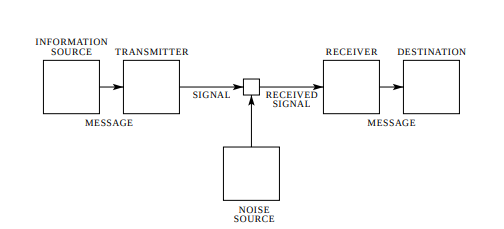
\includegraphics[width=0.65\textwidth]{comunicadorshannon.png}
  \begin{tikzpicture}
    \matrix (A) [matrix of nodes,
    column sep=25pt,
    row sep=30pt,
    nodes={minimum size=35pt}]
    {
      \node[label={[labelst]above:Fonte de\\informação},blocoq] (fonte) {}; &
      \node[label={[labelst]above:Transmissor},blocoq] (trans) {}; &
      \node[minimum size=10pt,blocoq] (conn) {}; &
      \node[label={[labelst]above:Receptor},blocoq] (rec) {}; &
      \node[label={[labelst]above:Destino},blocoq] (dest) {}; \\
      & & \node[label={[labelst]below:Fonte de \\ruído},blocoq] (ruido) {}; \\
    };
    \draw[conecta] (fonte) -- node[pos=0.5,below,labelst,yshift=-20pt] {Mensagem} (trans);
    \draw[conecta] (trans) -- node[pos=0.5,below,labelst] {Sinal} (conn);
    \draw[conecta] (conn) --  node[pos=0.5,below,labelst] {Sinal\\recebido} (rec);
    \draw[conecta] (rec) -- node[pos=0.5,below,labelst,yshift=-20pt] {Mensagem} (dest);
    \draw[conecta] (ruido) -- (conn);
  \end{tikzpicture}
  \fonte{Adaptado de \textcite[p. 380]{MTC}.}
\end{figure}

De acordo com  a TMC, um \textit{gerador de informação} é um objeto capaz de produzir um conjunto $X$ de $n$ eventos com probabilidade de ocorrência $P(X)$, enquanto um \textit{receptor} possui um conjunto $Y$, também com $n$ eventos, com probabilidades associadas $P(Y)$. Durante a transmissão é possível que parte da informação seja perdida devido a ocorrência de ruídos, o que resulta diretamente na modificação dos valores de probabilidade dos elementos recebidos do conjunto $Y$. Reconhecendo portanto os elementos de $X$ e suas probabilidades associadas, espera-se que uma mensagem bem transmitida, ou seja, sem interferência de ruídos, seja aquela cujas probabilidades dos elementos do conjunto $Y$ sejam as mesmas dos elementos do conjunto $X$. Assim, se essas probabilidades forem distintas, podemos concluir que houve perda de informação na transmissão \cite{mathematical}.

Como na MQ, não sabemos o estado de um qubit até que uma medida seja aplicada e não é possível recuperar um estado após a medida deste, identificar a presença de um ruído torna-se mais complicado do que na transferência de informação clássica. Chamamos de decoerência o processo pelo qual um sistema quântico interage com o ambiente e perde sua coerência quântica, ou seja, sua capacidade de apresentar estados de superposição e entrelaçamento originais. Alguns autores como \textcite{chuang}, utilizam o termo decoerência como sinônimo de ruído quântico.

Os qubits, como unidades básicas de informação em sistemas quânticos, podem ser afetados por diferentes tipos de ruídos que comprometem a coerência dos estados quânticos, causando erros nas operações e nos resultados das medições. Alguns dos principais tipos de ruído que atuam sobre qubits são:
\begin{description}
\item [Ruído térmico:] é causado pela interação dos qubits com o ambiente, que gera flutuações de temperatura e pressão ao redor dos qubits, comprometendo sua estabilidade e aumentando as taxas de erros nos cálculos.

\item [Ruído de decoerência:] é causado por interações indesejadas entre os qubits e outras partículas que compõem o ambiente, como fótons, átomos e elétrons. Essas interações podem resultar em mudanças na fase e na amplitude dos estados quânticos, prejudicando a coerência dos qubits.

\item [Ruído de controle:] é causado por erros nas operações de controle dos qubits, que podem levar a variações imprevisíveis nas oscilações e nos estados dos qubits.

\item [Ruído de leitura:] é causado pelas imprecisões nas medições dos estados quânticos, que podem ser influenciadas por fatores como a taxa de amostragem e a sensibilidade dos sensores.

\item [Ruído de acoplamento:] é causado pela interação entre qubits próximos, que podem interferir uns com os outros e afetar suas propriedades individuais, resultando em erros nos cálculos e nas medições.
\end{description}

Vale ressaltar que o estudo dos ruídos quânticos contribuem para conhecer os efeitos deste e estimar técnicas de correção para o sistema. Essas técnicas envolvem desde a escolha dos materiais e dos métodos de construção dos sistemas até a implementação de algoritmos de correção de erros e aprimoramento da qualidade das medições.

Segundo \textcite{teseufscar}, os principais tipos de ruídos associados à decoerência da informação quântica, ou seja, a sua alteração do estado original são:

\begin{description}
  \item [Inversão de bit (\textit{bitflip}):] esse ruído consiste essencialmente na inversão do estado dos qubits emaranhados, fazendo com que estes saiam de um chamado estado puro --- essencial para o fenomeno de emaranhamento --- para um estado misto.
  \item [Inversão de fase (\textit{phaseflip}):] inverte a fase da função de onda que representa os qubits emaranhados.
  \item [Inversão de bit e fase (\textit{bit-phase flip}):] inverte tanto o estado quanto a fase do qubit.
\end{description}

\clearpage